\documentclass[10pt, oneside]{article}

\usepackage[T1]{fontenc}
\usepackage[utf8]{inputenc}
\usepackage{polski}
\usepackage{indentfirst}
\usepackage{caption}
\usepackage{float}
\usepackage{tikz}
\usepackage{polski}
\usepackage{fancyhdr}
\usepackage{lastpage}
\usepackage{tcolorbox}
\usepackage{graphicx}

\title{Specyfikacja funkcjonalna programu WireWorld}
\author{Danuta Stawiarz, Katarzyna Stankiewicz}
\date{20 maja 2019 r.}

\pagestyle{fancy}
\fancyhf{} 
\lhead{}
\rhead{} 
	
\rfoot{
\begin{center} Strona \thepage \hspace{1pt} z \pageref{LastPage}
\end{center}
}


\begin{document}
\maketitle
\tableofcontents
\newpage	


\section {Informacje ogólne}

W projekcie zastosowany będzie wzorzec MVC (Model View Controller). Aby ułatwić pracę nad projektem oraz późniejsze modyfikacje, wprowadzony zostanie przejrzysty przydział poszczególnych plików do odpowiednich pakietów. 
W pakiecie models będą się znajdować klasy, które służą do wykonywania wszelkich operacji związanych z implementacją funkcjonalności automatu komórkowego.
W pakiecie View znajdą się wszystkie pliki .fxml odpowiedzialne za wygląd automatu komórkowego.
W pakiecie controllers będą zawarte kontrolery, służące do obsługi żądań użytkownika.

\section{Schemat działania programu}
Program reaguje bezpośrednio na komendy użytkownika. 

\begin{enumerate}
\item Pobranie od użytkownika informacji o parametrach początkowych gry - wariantu gry, który zostanie przeprowadzony (Wireworld lub Life). Inicjacja obiektu klasy Wireworld lub Life (rozszerzenie abstrakcyjnej klasy Game).
\item  Pobranie danych o wymiarach planszy lub ścieżki do pliku, na podstawie którego ma zostać utworzona rozgrywka oraz utworzenie obiektu typu Board oraz umieszczenie go w obiekcie klasy Wireworld lub Life.
\item Reakcje na bezpośrednie działania użytkownika:
	\begin {itemize}
	\item Start -  naciśnięcie tego przycisku uruchomi symulację, zostanie wywołana metoda Play(), która przeprowadza symulację,
	\item Generations - w przypadku naciśnięcia którejś ze strzałek, zostaje wywołana metoda klasy Game -  play() lub playBack(), które generują wygląd kolejnych siatek. Wynik symulacji 			zostanie wyświetlony na ekranie aplikacji,
	\item Board reset - nastąpi zresetowanie tablicy reprezentującej siatkę za pomocą funckji klasy Board - Reset Board poprzez zamianę w obiekcie obiektu klasy Board w klasie Game na nowoutworzony obiekt tego typu,
	\item Upload file - spowoduje wczytanie siatki ze stanami poszczególnych komórek poprzez utworzenie obiektu klasy BoardImport  i odczyt informacji z niego,
	\item Random fill -  spowoduje wywołanie metody klasy Board - randomFill() i  wypełnienie siatki looswymi wartościami,
	\item Save - spowoduje utworzenie obiektu klasy BoardExport i zapis stanu tablicy do pliku za pomocą funkcji tej klasy
\end{itemize}
\end {enumerate}

\section{Wzorzec projektowy}
W projekcie zastosowany będzie wzorzec MVC (Model View Controller). Aby ułatwić pracę nad projektem oraz późniejsze modyfikacje, wprowadzony zostanie przejrzysty przydział poszczególnych plików do odpowiednich pakietów. 
W pakiecie models będą się znajdować klasy, które służą do wykonywania wszelkich operacji związanych z implementacją funkcjonalności automatu komórkowego.
W pakiecie View znajdą się wszystkie pliki .fxml odpowiedzialne za wygląd automatu komórkowego.
W pakiecie controllers będą zawarte kontrolery, służące do obsługi żądań użytkownika.

\section{Opis modułów}
Program składa się z trzech głównych modułów odpowiedzialnych za prawidłowe działanie programu. Są to
\begin {itemize}
\item Model -  odpowiada za przeprowadzanie kolejnych generacji, jak i całej symulacji
\item Files - moduł odpowiadający za obsługę plików tekstowych, z których możliwy jest odczyt i zapis informacji dotyczących parametrów gry
\item GUI - moduł odpowiadający za aspekt wizualny gry, a także reakcję na działania użytkownika (przekazuje informację o przypadkach naciśnięcia poszczególnych przycisków)
\end{itemize}

\subsection{Moduł Game}
Moduł ten odpowiada za poprawne przeprowadzenie symulacji. Zawiera klasy reprezentujące grę i zawierające w sobie obiekty klas będących składowymi innych modułów.
Klasy:

\begin{enumerate}
\item \textbf{Abstract Class Game()} - klasa ta stanowi podstawę dla klas dziedziczących po niej - Wireworld oraz Life, związane jest to z wariantem gry, który wybierze użytkownik. 
					Klasa ta zawiera obiekt klasy Board, który reprezentuje siatkę komórek.
					Główne metody tej klasy to:
	\begin{itemize}
	\item public  setCell(int stan) - umożliwia zmianę stanu wybranej komórki w siatce
	\item public getBoard() - zwraca obiekt klasy Board reprezentujący siatkę,
	\item public  setBoard(Board board) - pobiera obiekt klasy Board i zapisuje w zmiennej board,
	\item public update(Board board) - pobiera obiekt klasy Board i nadpisuje go w miejscu zmiennej board,
	\item public play() - metoda ta jest nadpisywana w klasach dziedziczących po klasie Game, odpowiada za przeprowadzenie symualacji w kierunku chronologicznym (generacja kolejnych stanów siatki) zgodnie z zasadami danego wariantu gry,
	\item public playBack()- metoda ta jest nadpisywana w klasach dziedziczących po klasie Game, odpowiada za przeprowadzenie symualacji w kierunku odwrotnym (generacja poprzednich stanów siatki) zgodnie z zasadami danego wariantu gry.
 
	\end{itemize}
	

\item   \textbf{public class Wireworld extends Game} - klasa ta jest pochodną klasy Game, następuje w niej przeciążenie metody play oraz play\_back. Zostają one dostosowane do zasad gry. 
\item  \textbf{ public class Wireworld extends Game} - klasa ta jest pochodną klasy Game, następuje w niej przeciążenie metody play oraz play\_back. Zostają one dostosowane do zasad gry. 
\end{enumerate}


\subsection{Moduł Model}
Moduł ten zawiera klasy będące składowymi klasy Game. Umożliwiają one przeprowadzenie szczegółowej symulacji. Najważniejsze klasy tego modułu to:
\begin {enumerate}
\item  \textbf{ public class Cell} - klasa reprezentująca pojedynczą komórkę. Główne zmienne zawarte w tej klasie to:
	\begin{itemize}
		\item private double x, private double y - zmienne określające położenie komórki w siatce,
		\item private double size -  wielkość komórki,
		\item private int state -  określa stan komórki, w zależności od wariantu gry komórka może znajdować się w dwóch lub czterech różnych stanach,
		\item private int aliveNextCells - określa ilość żywych sąsiadów w najbliższym otoczeniu komórki zgodnie z zasada sąsiedztwa Moore'a,
	\end{itemize}
	
	Klasa zawiera następujące metody:
	\begin{itemize}
	\item public double getX() - zwraca wartość zmiennej \texttt{x},
	\item public void setX(double)  ustawia wartość zmiennej \texttt {x} na wartość podaną jako argument wywołania metody,
	\item public double getY() - zwraca wartość zmiennej \texttt{y},
	\item  public void setY(double) - ustawia wartość zmiennej \texttt{y}  na wartość podaną jako argument wywołania metody,
	\item  public double getSize() - zwraca wartość zmiennej \texttt{size},
	\item public int getState(int) -zwraca watość zmiennej \texttt{state},
	\item public void setState(int) - ustawia stan komórki na wartość podaną przy wywołaniu metody,
	\item public void setAliveNextCells(int) - ustawia wartość zmiennej \texttt {aliveNextCells} na wartość podaną przy wywołaniu metody
	\end{itemize}

	Klasa Cell posiada również kilka konstruktorów, są to:
	\begin{itemize}
	\item public Cell() - przy braku argumentów, wartość zmiennej \texttt{state} będzie wynosiła 0,
	\item public Cell (Cell cell) - przy tworzeniu obiektu jako argument zostaje podany obiekt klasy Cell - zmienna \texttt{state} otrzymuje taką wartość, jak wartość zmiennej \texttt {state} obiektu 
	\end{itemize}


\item  \textbf{ public class Board} -klasa ta reprezentuje siatkę komórek i jest jedną z najważniejszych klas. Zawiera następujące zmienne:
\begin{itemize}
	\item private int columns - zmienna oznaczająca liczbę kolumn w siatce,
	\item private int rows - zmienna oznaczająca liczbę wierszy w siatce,
	\item Cell[] cells - tablica obiektów klasy Cells reprezentująca siatkę komórek
\end{itemize}
 
Klasa ta posiada następujące główne metody:
\begin {itemize}
	\item public void countNeighbours()  - metoda zliczająca sąsiadów o stanie określonym jako "żywa" dla każdej komórki w siatce i przypisująca obliczoną wartość do zmiennej \texttt{aliveNextCells} w obiektach klasy Cells (metoda dla wariantu gry Life).
		\item public void countHeadNeighbours()  - metoda zliczająca sąsiadów o stanie określonym jako Głowa Elektronu dla każdej komórki w siatce i przypisująca obliczoną wartość do zmiennej \texttt{aliveNextCells} w obiektach klasy Cells (metoda dla wariantu Wireworld).
	\item public Cell getCell (int,int) - zwraca obiekt klasy Cell umieszczony w siatce pod wskazanymi w wywołaniu współrzędnymi,
	\item public void setCell (int,int,int) - przypisuje pod podane współrzędne komórkę o określonym stanie, metoda jest przeciążana,
	\item public void setCell(Cells) - przypisuje podaną w argumencie wywołania komórkę pod adres w tablicy.
\end{itemize}	
	
Klasa ta posiada także kilka konstruktorów:
\begin {itemize}
\item public Board() - pusty konstruktor, zostaje w nim utworzona pusta tablca obiektów Cells, o wymiarach domyślnych,
\item public Board(Board board) - konstruktor, w którym nowopowstały obiekt przejmuje parametry obiektu podanego w argumenatch wywołania.
\end{itemize}
\end{enumerate}

\subsection{Moduł Controller}
Moduł ten odpowiada za obsługę przez program plików tekstowych. Użytkownik ma możliwość otworzenia symulacji przez wczytanie jej parametrów do pliku, a także jej późniejszy zapis. Wymaganiom tym odpowiadają dwie klasy:
\begin {enumerate}
\item \textbf{BoardExport} - klasa ta odpowiada za zapis pliku danych dotyczących siatki komórek. Korzysta z biblioteki java.io.*.  Posiada zmienne:
\begin{itemize}
\item Filereader file - plik, dp którego znak po znaku zostaną zapisane dane
\end{itemize}
Metodą tek klasy jest:
\begin{itemize}
\item public void Save(Board board) - przekazany do metody obiekt typu Board, zostaje zapisany do pliku, poprzez zapis poszczególnych danych dotyczących wymiarów siatki, położenia i stanów poszczególnych komórek
\end{itemize}


\item \textbf{BoardImport} - klasa ta odpowiada za odczyt z pliku danych dotyczących siatki komórek. Korzysta z biblioteki java.io.*.  Posiada zmienne:
\begin{itemize}
\item Filereader file - plik, z którego znak po znaku zostaną odczytane dane
\end{itemize}
Metodą tek klasy jest:
\begin{itemize}
\item public BoardRead() - w metodzie tej następuje odczytanie poszczególych danych z pliku. Zwraca obiekt klasy Board.
\end{itemize}
\end{enumerate}

\subsection{Moduł View}
W module view znajduje się plik Game.fxml, który zawiera kod implementacji interfejsu użytkownika w javaFX dla Automatu Komórkowego.

\section{Zastosowane algorytmy}
W programie zostały zastosowane następujące algorytmy:


\subsection{ Algorytm wyznaczania stanu komórki dla wariantu gry Life}
	\begin {enumerate}
	\item Wywołanie metody klasy Board dla konkretnej komórki w celu zliczenia jej żywych sąsiadów.
	\item Określenie stanu komórki na podstawie ilości jej żywych sąsiadów:
		\begin{itemize}
		\item Komórka martwa -jeżeli  liczba żywych sąsiadów wynosi 3, stan komórki zostaje określony jako "żywa", w innym wypadku komórka pozostaje martwa;
		\item Komórka żywa - jeżeli liczba żywych komórek wynosi 2 lub 3, stan nie zmienia się , w innym wypadku komórka pozostaje martwa.
		\end{itemize}
	\item Zapis nowej wartości stanu komórki w obiekcie klasy Cells pod zmienną \texttt{state}.
	\end {enumerate}


\subsection{ Algorytm wyznaczania stanu komórki dla wariantu gry Wireworld}
	\begin {enumerate}
		\item Wywołanie metody klasy Board zliczającej sąsiednich komórek, których stan określany jest jako Głowa Elektronu. 
		\item Określenie stanu komórki na podstawie poprzedniego stanu i analizy stanów sąsiednich komórek.
		\begin{itemize}
		\item Komórka pozostaje Pusta, jeśli była Pusta.
		\item Komórka staje się Ogonem elektronu, jeśli była Głową elektronu.
		\item Komórka staje się Przewodnikiem, jeśli była Ogonem elektronu.
		\item Komórka staje się Głową elektronu tylko wtedy, gdy dokładnie 1 lub 2 sąsiadujące komórki są Głowami Elektronu.
		\item Komórka staje się Przewodnikiem w każdym innym wypadku
	\end{itemize}
	\item Zapis nowej wartości stanu komórki w obiekcie klasy Cells pod zmienną \texttt{state}.
	
\end {enumerate}
Dla obu algorytmów wykorzystane jest sąsiedztwo Moore'a. 

\section{Diagram klas}

\begin{figure}[H]
	\centering
	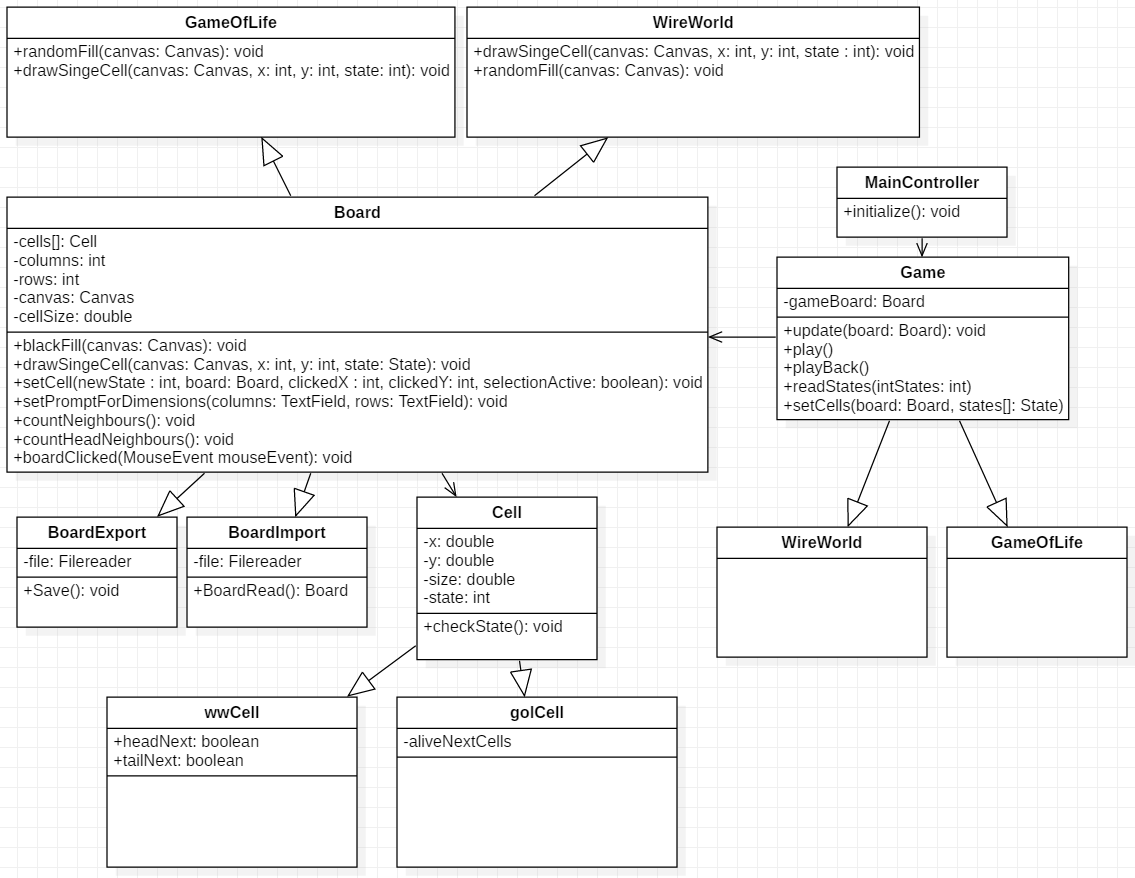
\includegraphics[width=13cm]{DiagramKlas.png}
	\caption{Diagram Klas}
\end{figure}

\section{Testy}
\subsection{Test klasy Cells}
W celu przetestowania tej klasy należy utworzyć jej obiekt oraz poprzez wywołania kolejnych metod sprawdzić, czy jej zmienne są poprawnie inicjowane. Szerszych testów wymaga modułu zliczjący żywych sąsiadów lub sąsiadów o określonym stanie w zależności od wariantu gry, w którym ma funkcjonować obiekt.
\subsection{Test klasy Board}
Test tego modułu zakłada zainicjowanie obiektu klasy Board oraz przetestowanie działania jego metod. Do przetestowania tego modułu potrzebny jest poprawnie działająca klasa Cells. Szczegółowych testów wymaga metoda \texttt{neighbours} oraz \texttt{neighbours2}.
\subsection{Test modułu Files}
Testy tego modułu polegają na odczycie i zapisie do plików txt. W celu przetestowania tego modułu niezbędny jets poprawnie działający moduł Board. Zapis do pliku w przypadku gry Life powinien wyglądac następująco:
\begin {verbatim}
5 5 
1 0 1 0 0
0 0 0 0 0
1 0 0 1 0
0 1 1 1 1
0 0 0 0 0 
\end{verbatim}
Pierwsze dwie cyfry oznaczają tu wymiary tablicy, która jest zmienną w obiekcie klasy typu Board. Kolejne cyfry symbolizują stany poszczególnych komórek (obiektów klasy Cells), które zostają zainicjowane w tablicy w obiekcie klasy Board. Zera oznaczają stan komórki jako "martwa", a jedynki jako "żywa".
Plik przedstawiający siatkę dla wariantu gry "Wireworld" powinien wyglądać następująco:
\begin {verbatim}
5 5 
1 0 1 3 0
0 0 0 0 2
1 0 0 1 0
0 1 1 1 1
2 0 0 3 0 
\end{verbatim}
Pierwsze dwie cyfry oznaczają tu wymiary tablicy, która jest zmienną w obiekcie klasy typu Board. Kolejne cyfry symbolizują stany poszczególnych komórek (obiektów klasy Cells), które zostają zainicjowane w tablicy w obiekcie klasy Board. Zera oznaczają stan komórki jako "pusta",  jedynki jako "głowa elektronu", dwójki jako "ogon elektronu", a trójki jako "przewodnik".

\subsection {Test modułu View}
Test polega na sprawdzeniu sfery wizualnej oraz reakcji programu na poszczególne działania użytkowników (przypadki naciśnięcia przynicku lub wpisania tekstu).




\end{document}